%中間審査概要テンプレート ver. 3.0

\documentclass[uplatex,twocolumn,dvipdfmx]{jsarticle}
\usepackage[top=22mm,bottom=22mm,left=22mm,right=22mm]{geometry}
\setlength{\columnsep}{10mm}
\usepackage[T1]{fontenc}
\usepackage{txfonts}
\usepackage[expert,deluxe]{otf}
\usepackage[dvipdfmx,hiresbb]{graphicx}
\usepackage[dvipdfmx]{hyperref}
\usepackage{pxjahyper}
\usepackage{secdot}





%タイトルと学生番号,名前だけ編集すること
\title{\vspace{-5mm}\fontsize{14pt}{0pt}\selectfont RedPenを用いた文書自動検査システムの導入}
\author{\normalsize プロジェクトマネジメントコース 矢吹研究室 1442031 氏名 小山隆太郎}
\date{}
\pagestyle{empty}
\begin{document}
\fontsize{10.5pt}{\baselineskip}\selectfont
\maketitle





%以下が本文
\section{背景}
RedPen\cite{a}とは,技術文書をターゲットにした文書自動検査ツールであり,説明書やマニュアル,論文,仕様書等の検査をするのに用いられる.また,様々な言語(英語,日本語,中国語など)の検査にも適用できる.RedPenはオープンソースのプロジェクトで,現在もコードの追加,改変が行われている\cite{b}.技術文書には全ての読者が同一の意図を読み取る必要があり,日記等と違い自分以外の第三者が読むため,恥ずかしくない文書を書かなければならない.恥ずかしい文書には,文中に利用する記号や専門用語が統一されていない場合や,”誰がが行く”のように,明らかな文章の間違いが多数存在する.また,”だから””かなり”といった口語が混じってしまうと,文書の品質が落ちることにつながる.
これらの文書表現は,学生が書く卒論や課題等の文書作成においても注意しなければならない.このような状況に対して,RedPenを作成環境に導入することで,文書の品質が向上すると考えた.

\section{目的}
RedPenの文書添削の結果には,正しい文書表現であるが,間違いだと指摘されることがある.また,誤った文書を添削しないこともあるため,どのような文書でも正しい文書添削が行えるマシンを構築し,プロジェクトで運用することを目的とする.

\section{手法}
RedPenは組織のルール(学校,会社等)に対応できるように設定が柔軟に行える仕様となっている\cite{c}.同一設定で文書の添削を繰り返し,RedPenの添削結果の推移,要素をまとめる.この結果から,添削機能の追加,変更を行う.

\section{想定される成果物}
個人または複数人プロジェクトで活用できる文書添削システムを構築する.

\section{進捗状況}
矢吹研究室に所属する3年生の課題文の添削を行い,マシンの添削結果の推移を観察した.この結果から添削機能に不十分な要素をまとめた.
\begin{figure}[h]
\centering
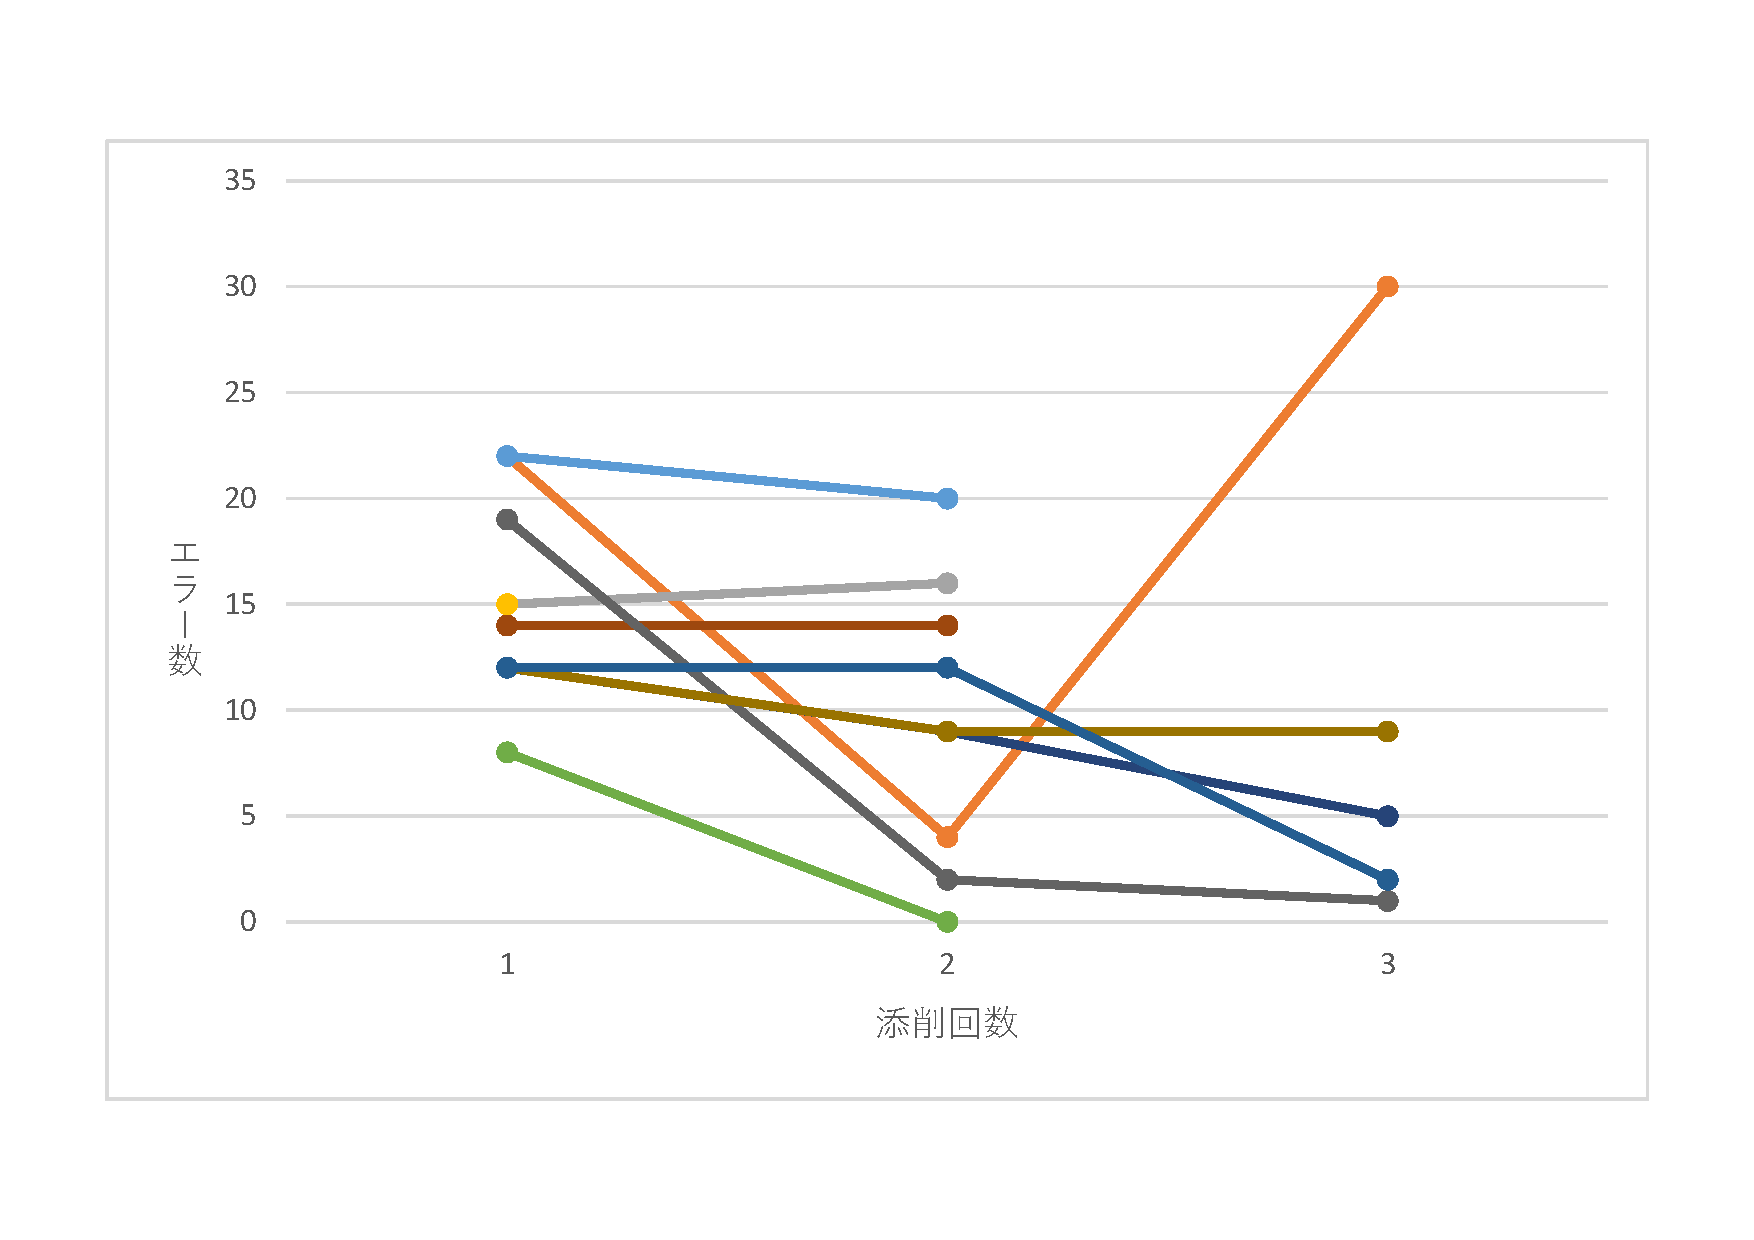
\includegraphics[width=8cm,clip]{images.pdf}
\caption{同一設定での添削結果と減る推移}\label{サンプル図}
\end{figure}

\begin{enumerate}
 \item 文長が長すぎる添削結果が多くを占め,論文向けの文長に設定を考察する必要がある
 \item 助詞が連続して使われると,正しい文書や名詞中の同文字も助詞とみなされ添削対象に含まれる
 \item 4文字以上の漢字は助詞を使用し分割しなければならない
\end{enumerate}

\section{今後の計画}
\begin{enumerate}
 \item 組織ごとに文書に必要になる要素をまとめる
 \item Javascriptを用いて添削機能の追加を行う
 \item 文書作成に利用してもらう
\end{enumerate}


\bibliographystyle{junsrt}
\bibliography{biblio}%「biblio.bib」というファイルが必要.

\end{document}
